\documentclass[journal,10pt]{IEEEtran}
\usepackage{amsmath,amssymb}
\usepackage{graphicx,array,url}
\usepackage{balance}
\usepackage{tikz}
\usetikzlibrary{arrows.meta,fit,backgrounds}
\usepackage[hidelinks]{hyperref}
\begin{document}
\title{Embedded Assamese Scene-Text Recognition\\and English Translation on Jetson}
\author{Monor~Enghi, Anjan~Kumar~Talukdar, and Navajit~Saikia%
\thanks{M. Enghi and A. K. Talukdar are with the Department of Electronics and Communication Engineering, Gauhati University, Gopinath Bordoloi Nagar, Guwahati 781014, Assam, India (e-mail: monorenghi@gmail.com; anjantalukdar@gauhati.ac.in).}%
\thanks{N. Saikia is with Assam Engineering College, Jalukbari, Guwahati 781013, Assam, India (e-mail: navajit.ete@aec.ac.in).}}
\maketitle
\begin{abstract}
Deploying Assamese scene-text reading on an embedded device requires coordinated detection, recognition, translation, and camera processing within a shared resource budget. This letter extends our accepted conference framework through a Jetson Orin Nano implementation with CUDA-accelerated ONNX inference, latest-frame selection, and asynchronous offline English translation. A translation-enabled live camera observation achieves 8.367 processed frames/s, with 1651.92~MiB peak sampled application RSS and 9.18~W mean module power under an existing-cache workload. An OCR-only replay of four synthetic scenes achieves $4.601\pm0.011$ frames/s across three repeats, providing a 5.09-fold throughput increase over CPU execution. Functional checks on three words in two real photographs verify localization, transcription, and bilingual-consistent English output. The results characterize embedded execution, memory use, and translation behavior, complementing the model-development study with measured device-level evidence.
\end{abstract}
\begin{IEEEkeywords}
Assamese scene text, embedded vision, Jetson Orin Nano, ONNX Runtime, offline translation.
\end{IEEEkeywords}

\section{Introduction}
\IEEEPARstart{A}{ssamese} text on signs, storefronts, posters, and other natural-scene surfaces carries information that a portable reading system must locate, transcribe, and translate. For an embedded implementation, the challenge extends beyond neural inference: camera transport, crop processing, Unicode rendering, and translation compete for processor time and memory. A deployable system must coordinate these stages while keeping the displayed result responsive to the current scene.

Our earlier work, ``Design of a Natural Scene Assamese Text Recognition System,'' develops a YOLO11n detector and VGG--SVTRv2/CTC recognizer with a translation interface~\cite{prior}. That manuscript was accepted at the 11th National Conference on Computer Vision, Pattern Recognition, Image Processing and Graphics, held at LNMIIT Jaipur on July~22--24, 2026; its proceedings are not yet published. It establishes the model-development framework using collected Assamese scene images and synthetic text crops generated with SynthTIGER~\cite{synthtiger}. Its translation interface uses \texttt{deep-translator}, with speech output through gTTS.

This letter extends that framework to embedded execution. The contribution comprises (i) a host-camera/container inference boundary with latest-frame replacement, (ii) CUDA OCR coordinated with a local CPU INT8 English translation model and exact-source cache, and (iii) measured throughput, memory, module power, and publication-age characterization on Jetson Orin Nano. Translation runs locally without an external translation service. The extension evaluates system integration and resource behavior; the conference study supplies the model-development context rather than a device-performance baseline.

\section{Model and Deployment Configuration}
Scene-text recognizers include CTC-based methods such as SVTRv2~\cite{svtrv2} and context-aware approaches such as PARSeq, which uses permutation language modeling~\cite{parseq}.

The system maps a scene image $I$ to ordered text regions $\{(b_i,\hat{s}_i)\}_{i=1}^{R}$ and their English translations. We distinguish localization, crop transcription, and end-to-end spotting following the task separation in the Robust Reading Competition~\cite{rrc2015}. Exact-text spotting requires both a matching region and a matching transcription. The deployed detector is identified by its ONNX metadata as YOLO11n with a single Assamese-text class and a $640\times640$ input.

The recognizer follows the VGG/transformer/CTC design used in the preceding framework~\cite{prior,svtrv2,ctc}. Inspection of the deployed ONNX graph identifies eight backbone blocks and a 143-symbol output. The runtime resizes RGB crops to $128\times32$, normalizes pixel values to $[-1,1]$, and applies greedy CTC decoding. Consecutive repeated symbols are collapsed and blanks removed; blanks between identical symbols preserve both characters. This deployed configuration is distinguished from the twelve-layer, 159-class configuration described in the conference manuscript. We report the exported model's actual interface and measure its device execution, without transferring earlier recognition scores to this configuration.

ONNX Runtime~\cite{ort} requests CUDA followed by CPU for OCR, while translation uses CPU. Startup checks verify the requested providers and reject CPU-only session fallback in CUDA mode. Detection and recognition graphs occupy 10\,583\,484 and 57\,329\,274 bytes, respectively, totaling 64.77~MiB; translation weights and runtime allocations are additional. Model hashes and software metadata are retained with the experiment records.

\section{Embedded Pipeline}
\subsection{Camera Transport and Latest-Frame Processing}
The host captures CSI images at $1920\times1080$ and a configured rate of 30~frames/s using \texttt{nvarguscamerasrc}~\cite{jetson}, NVIDIA image conversion, and quality-85 JPEG encoding. A loopback TCP sender feeds the inference container, avoiding dependence on container camera plugins. A receiver thread reconstructs JPEG images across socket reads and replaces a single latest-complete-frame slot. Sequence identifiers allow the inference worker to select each new frame once. A 16~MiB guard limits incomplete-frame accumulation.

The inference worker decodes the selected image, detects regions, orders crops, recognizes text, submits source strings for translation, and renders the current Assamese and available English outputs. A shared quality-80 JPEG publication buffer serves browser viewers. Figure~\ref{fig:architecture} shows these execution boundaries. Host capture and OCR are decoupled, and multiple viewers share one inference worker.

\begin{figure}[t]
\centering
% Native vector diagram. Coordinates are in centimetres; no raster assets.
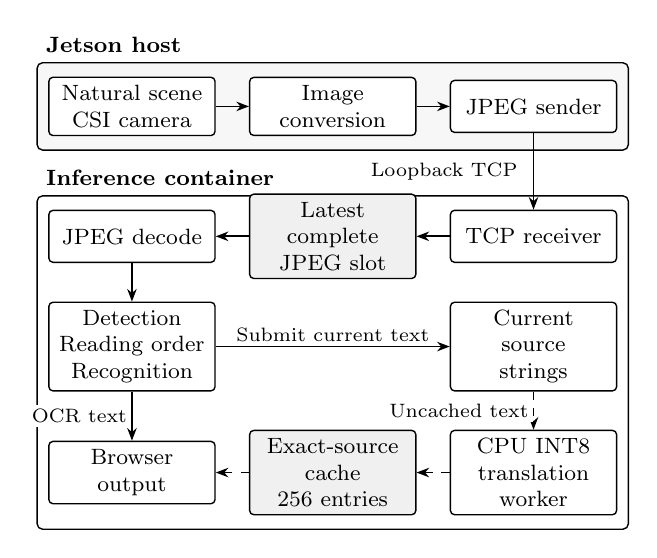
\begin{tikzpicture}[
  font=\footnotesize,
  block/.style={draw, rounded corners=1.5pt, line width=0.5pt,
    fill=white, align=center, text width=1.90cm,
    minimum height=0.66cm, inner sep=3pt},
  flow/.style={-{Stealth[length=1.6mm]}, line width=0.65pt},
  async/.style={flow, dashed},
  note/.style={font=\scriptsize, fill=white, inner sep=1.5pt},
  boundary/.style={draw, rounded corners=2pt, line width=0.5pt,
    inner xsep=4pt, inner ysep=5pt}
]
% Host camera stages.
\node[block] (camera) at (0,0) {Natural scene\\CSI camera};
\node[block] (convert) at (2.55,0) {Image conversion};
\node[block] (sender) at (5.10,0) {JPEG sender};
\draw[flow] (camera) -- (convert);
\draw[flow] (convert) -- (sender);

% Receiver progresses independently of the OCR consumer.
\node[block] (receiver) at (5.10,-1.65) {TCP receiver};
\node[block, fill=black!6] (slot) at (2.55,-1.65)
  {Latest complete\\JPEG slot};
\node[block] (decode) at (0,-1.65) {JPEG decode};
\draw[flow] (sender.south) --
  node[note, midway, anchor=east, xshift=-4pt] {Loopback TCP} (receiver.north);
\draw[flow] (receiver) -- (slot);
\draw[flow] (slot) -- (decode);

% OCR is published without waiting for the translation worker.
\node[block, minimum height=1.02cm] (ocr) at (0,-3.05)
  {Detection\\Reading order\\Recognition};
\node[block] (desired) at (5.10,-3.05) {Current source\\strings};
\draw[flow] (decode) -- (ocr);
\draw[flow] (ocr) -- node[note, above] {Submit current text} (desired);

\node[block] (browser) at (0,-4.65) {Browser output};
\node[block, fill=black!6] (cache) at (2.55,-4.65)
  {Exact-source cache\\256 entries};
\node[block] (translator) at (5.10,-4.65)
  {CPU INT8\\translation worker};
\draw[flow] (ocr) -- node[note, left] {OCR text} (browser);
\draw[async] (desired) -- node[note, left] {Uncached text} (translator);
\draw[async] (translator) -- (cache);
\draw[async] (cache) -- (browser);

% Execution boundaries are behind nodes and arrows.
\begin{scope}[on background layer]
  \node[boundary, fit=(camera)(sender), fill=black!3] (host) {};
  \node[boundary, fit=(decode)(receiver)(ocr)(desired)(browser)(translator)]
    (container) {};
\end{scope}
\node[font=\footnotesize\bfseries, anchor=south west]
  at (host.north west) {Jetson host};
\node[font=\footnotesize\bfseries, anchor=south west]
  at (container.north west) {Inference container};
\end{tikzpicture}

\caption{Embedded scene-text reading and translation pipeline. Dashed arrows denote asynchronous translation and cache lookup; recognition continues while English results become available.}
\label{fig:architecture}
\end{figure}

\subsection{Detection, Reading Order, and Recognition}
Images are letterboxed for detection, with confidence threshold~0.25 and nonmaximum-suppression IoU threshold~0.45. Crops are recognized sequentially. Geometric ordering groups approximately horizontal text into rows before sorting each row from left to right. For box~$i$, let $c_i$ be its vertical center and $h_i$ its height. A box joins the closest qualifying row, represented by median center $c_r$ and height $h_r$, when vertical overlap $o(i,r)$ satisfies
\begin{align}
o(i,r)&\geq \tfrac12\min(h_i,h_r),\\
|c_i-c_r|&\leq \tfrac12\min(h_i,h_r).
\end{align}
Scores are permuted with boxes so detector confidence remains associated with the correct crop. This rule supports horizontal reading order without a separate object-grouping stage.

\subsection{Translation model}
Low-precision inference is an established strategy for efficient on-device neural execution~\cite{quantization}. English translation uses an INT8 ONNX export of the distilled 200M IndicTrans2 Indic-to-English model~\cite{indictrans2,export}. A dedicated worker translates deduplicated source strings while OCR continues. Exact stripped source text keys the cache, preserving text-to-translation association as detections change. Success and failure maps each retain up to 256 entries; attempts are separated by 0.5~s, and failed strings have a 30~s retry delay. The CPU translator uses two intra-operation threads, a 256-token input limit, and at most 64 generation steps. Normalization and script conversion precede tokenization. Cached English output is reused when freshly recognized Assamese text matches an existing key.

\section{Publication Age and Workload}
Following the information-freshness perspective of age-of-information research~\cite{aoi}, we distinguish frame age from processing throughput. Let $a_k$ denote receiver arrival of complete JPEG~$k$, and $s_n$ inference selection time. Single-slot replacement selects
\begin{equation}
k(n)=\max\{k:a_k\leq s_n\}.
\end{equation}
For a continuously supplied stream with complete-frame interarrival bounded by $T_a$, the receiver-relative selection age satisfies
\begin{equation}
0\leq s_n-a_{k(n)}\leq T_a.
\end{equation}
If $T_p(n)$ covers decoding through output encoding, receiver-to-publication age is
\begin{equation}
A_n=(s_n-a_{k(n)})+T_p(n)\leq T_a+T_p(n).
\end{equation}
This conditional bound concerns the receiver slot; upstream sensor, encoding and socket delays are separate. Replacement avoids accumulating an application FIFO when processing is slower than arrival, at the cost of skipping intermediate frames. A FIFO comparison is outside the present measurements.

For $R_n$ detected regions, sequential recognition gives
\begin{equation}
T_p(n)\approx T_{\mathrm{fixed}}+\sum_{i=1}^{R_n}T_{\mathrm{rec},i}.
\end{equation}
Region density and rendering therefore affect throughput alongside neural inference. Asynchronous translation removes a direct generation wait from the OCR loop, while CPU, memory and thermal resources remain shared.

\section{Experimental Results}
\subsection{Platform and Measurement Protocol}
Experiments used an Orin Nano Super developer kit reporting 7.3~GiB RAM, L4T R39.2.1, and a 25~W power mode. The inference container used ONNX Runtime~1.23.0 with CUDA execution. Timestamped stage records and raw \texttt{tegrastats} logs preserve the measurement boundaries. The Tegrastats utility~\cite{tegrastats} samples module power, utilization and system RAM every 500~ms; application RSS is sampled separately. VDD\_IN denotes module power rather than wall-input power. Provider checks confirm CUDA-session availability; per-operator placement is not inferred from those checks. The Jetson container passed 57 regression tests, including metric-scope and timestamp-transport checks.

\subsection{Controlled OCR Replay}
Four AI-generated scene images provided a fixed computational workload for comparing full-size CUDA, reduced-size CUDA and full-size CPU execution. Each condition used three 60-second measured repeats following 30-second warmup intervals. Translation was disabled for this OCR ablation. Processing included PNG decoding, detection, reading order, recognition, annotation and JPEG encoding; the synthetic images were not used as recognition ground truth.

Full-size ($1536\times1024$) CUDA replay achieved $4.601\pm0.011$ frames/s, compared with $0.904\pm0.003$ on CPU, a 5.09-fold throughput increase. Reducing replay size to $960\times640$ raised CUDA throughput to $5.096\pm0.022$ frames/s, a 10.8\% increase. Values are means and sample standard deviations across repeats. The means of repeat-level processing p95 values were 258.19~ms for full-size CUDA, 231.24~ms for reduced-size CUDA, and 1468.39~ms for CPU. Full-size CUDA peak process RSS was 1283.75~MiB and mean sampled module power was 8.95~W. This comparison measures the complete OCR/rendering loop rather than detector inference alone.

\subsection{Real-Scene Functional Verification}
Two real photographs (Fig.~\ref{fig:real-scenes}) exercise a bilingual road sign and commercial signs. Manually specified bounding boxes and author-confirmed transcriptions define three readable Assamese/shared-script words. Latin and tiny or partial background text are excluded. A prediction is in scope when at least half its area lies inside a declared evaluation rectangle; one-to-one greedy matching uses IoU~$\geq0.5$. Exact-text spotting additionally requires an exact transcription after NFC normalization and whitespace collapse.

All three regions were detected and correctly spotted, giving precision, recall and H-mean of 1.00 within this scope. Ground-truth crops gave zero code-point CER over 18 reference code points and 3/3 exact words. The translated outputs matched the visible English MOHANBARI, TIBET and KITCHEN after casefolding. These checks verify the deployed components on the selected examples; they do not replace the corpus-level evaluation in the preceding model-development study. A spurious detection on Latin text falls outside the declared scope.

\begin{figure}[t]
\centering
\begin{minipage}[b]{0.56\columnwidth}
\centering
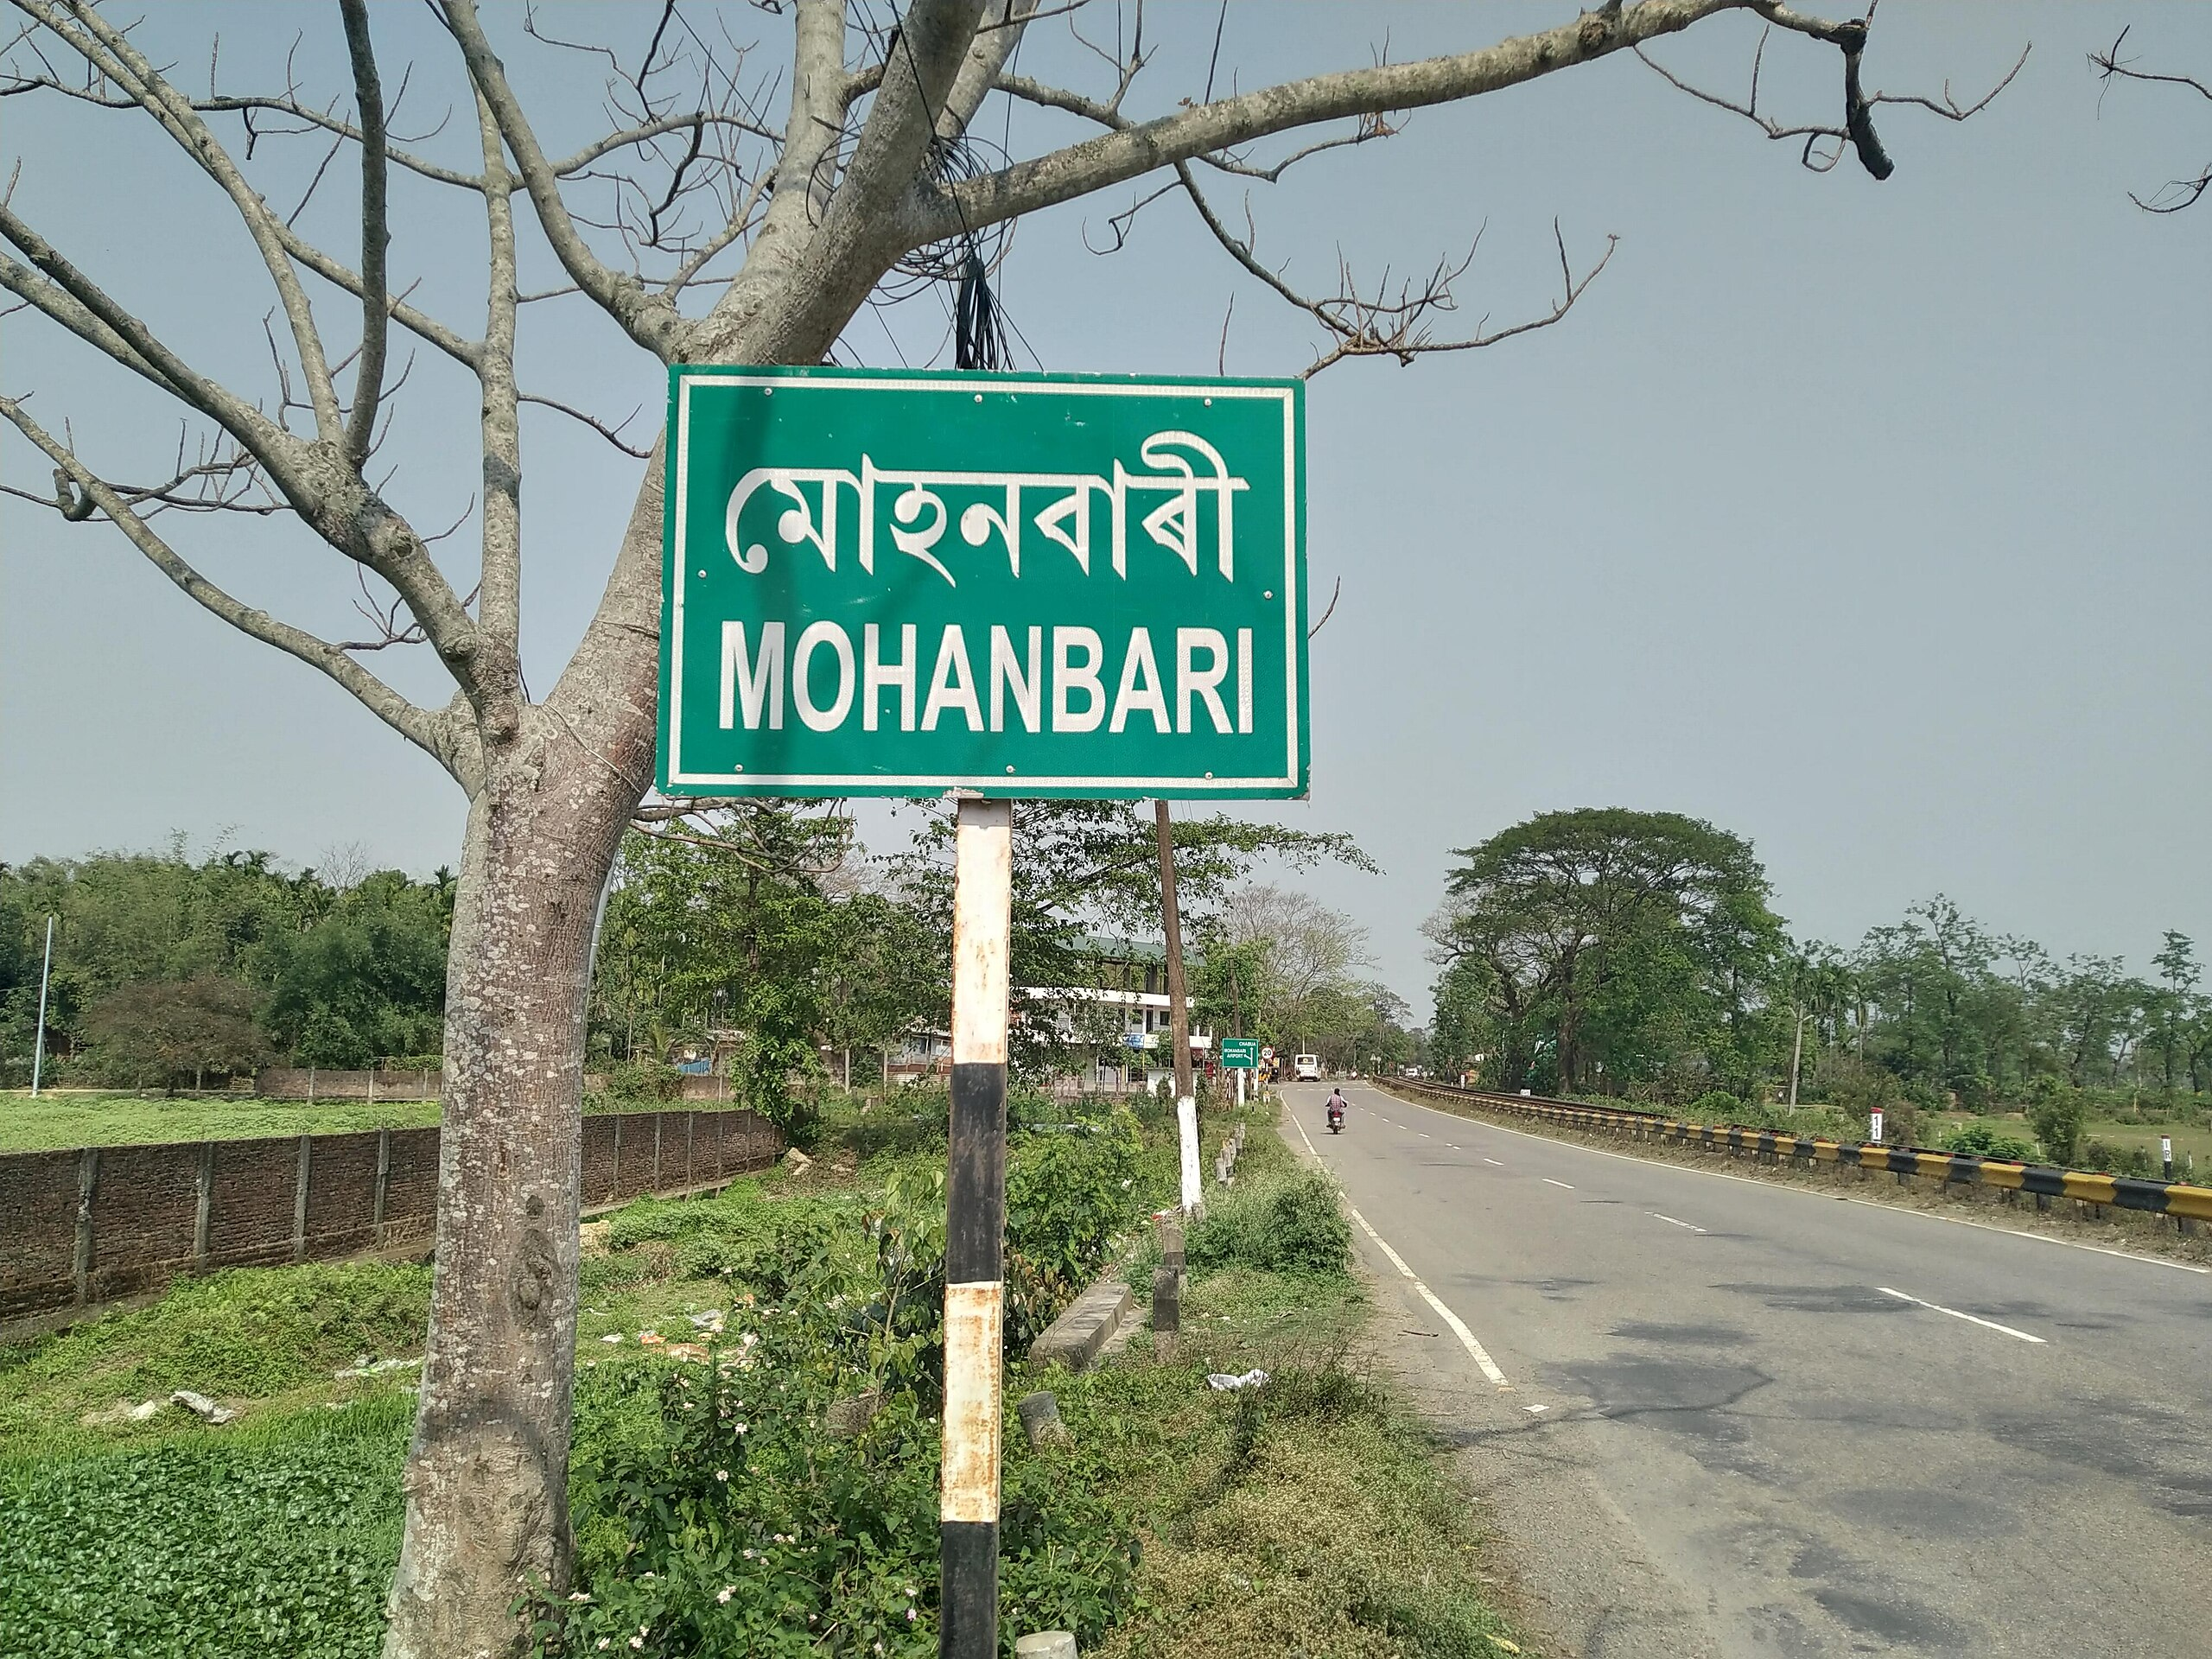
\includegraphics[width=\linewidth,height=1.45in,keepaspectratio]{../../experiments/real_scenes_v1/images/mohanbari.jpg}\\
\small (a)
\end{minipage}\hfill
\begin{minipage}[b]{0.42\columnwidth}
\centering
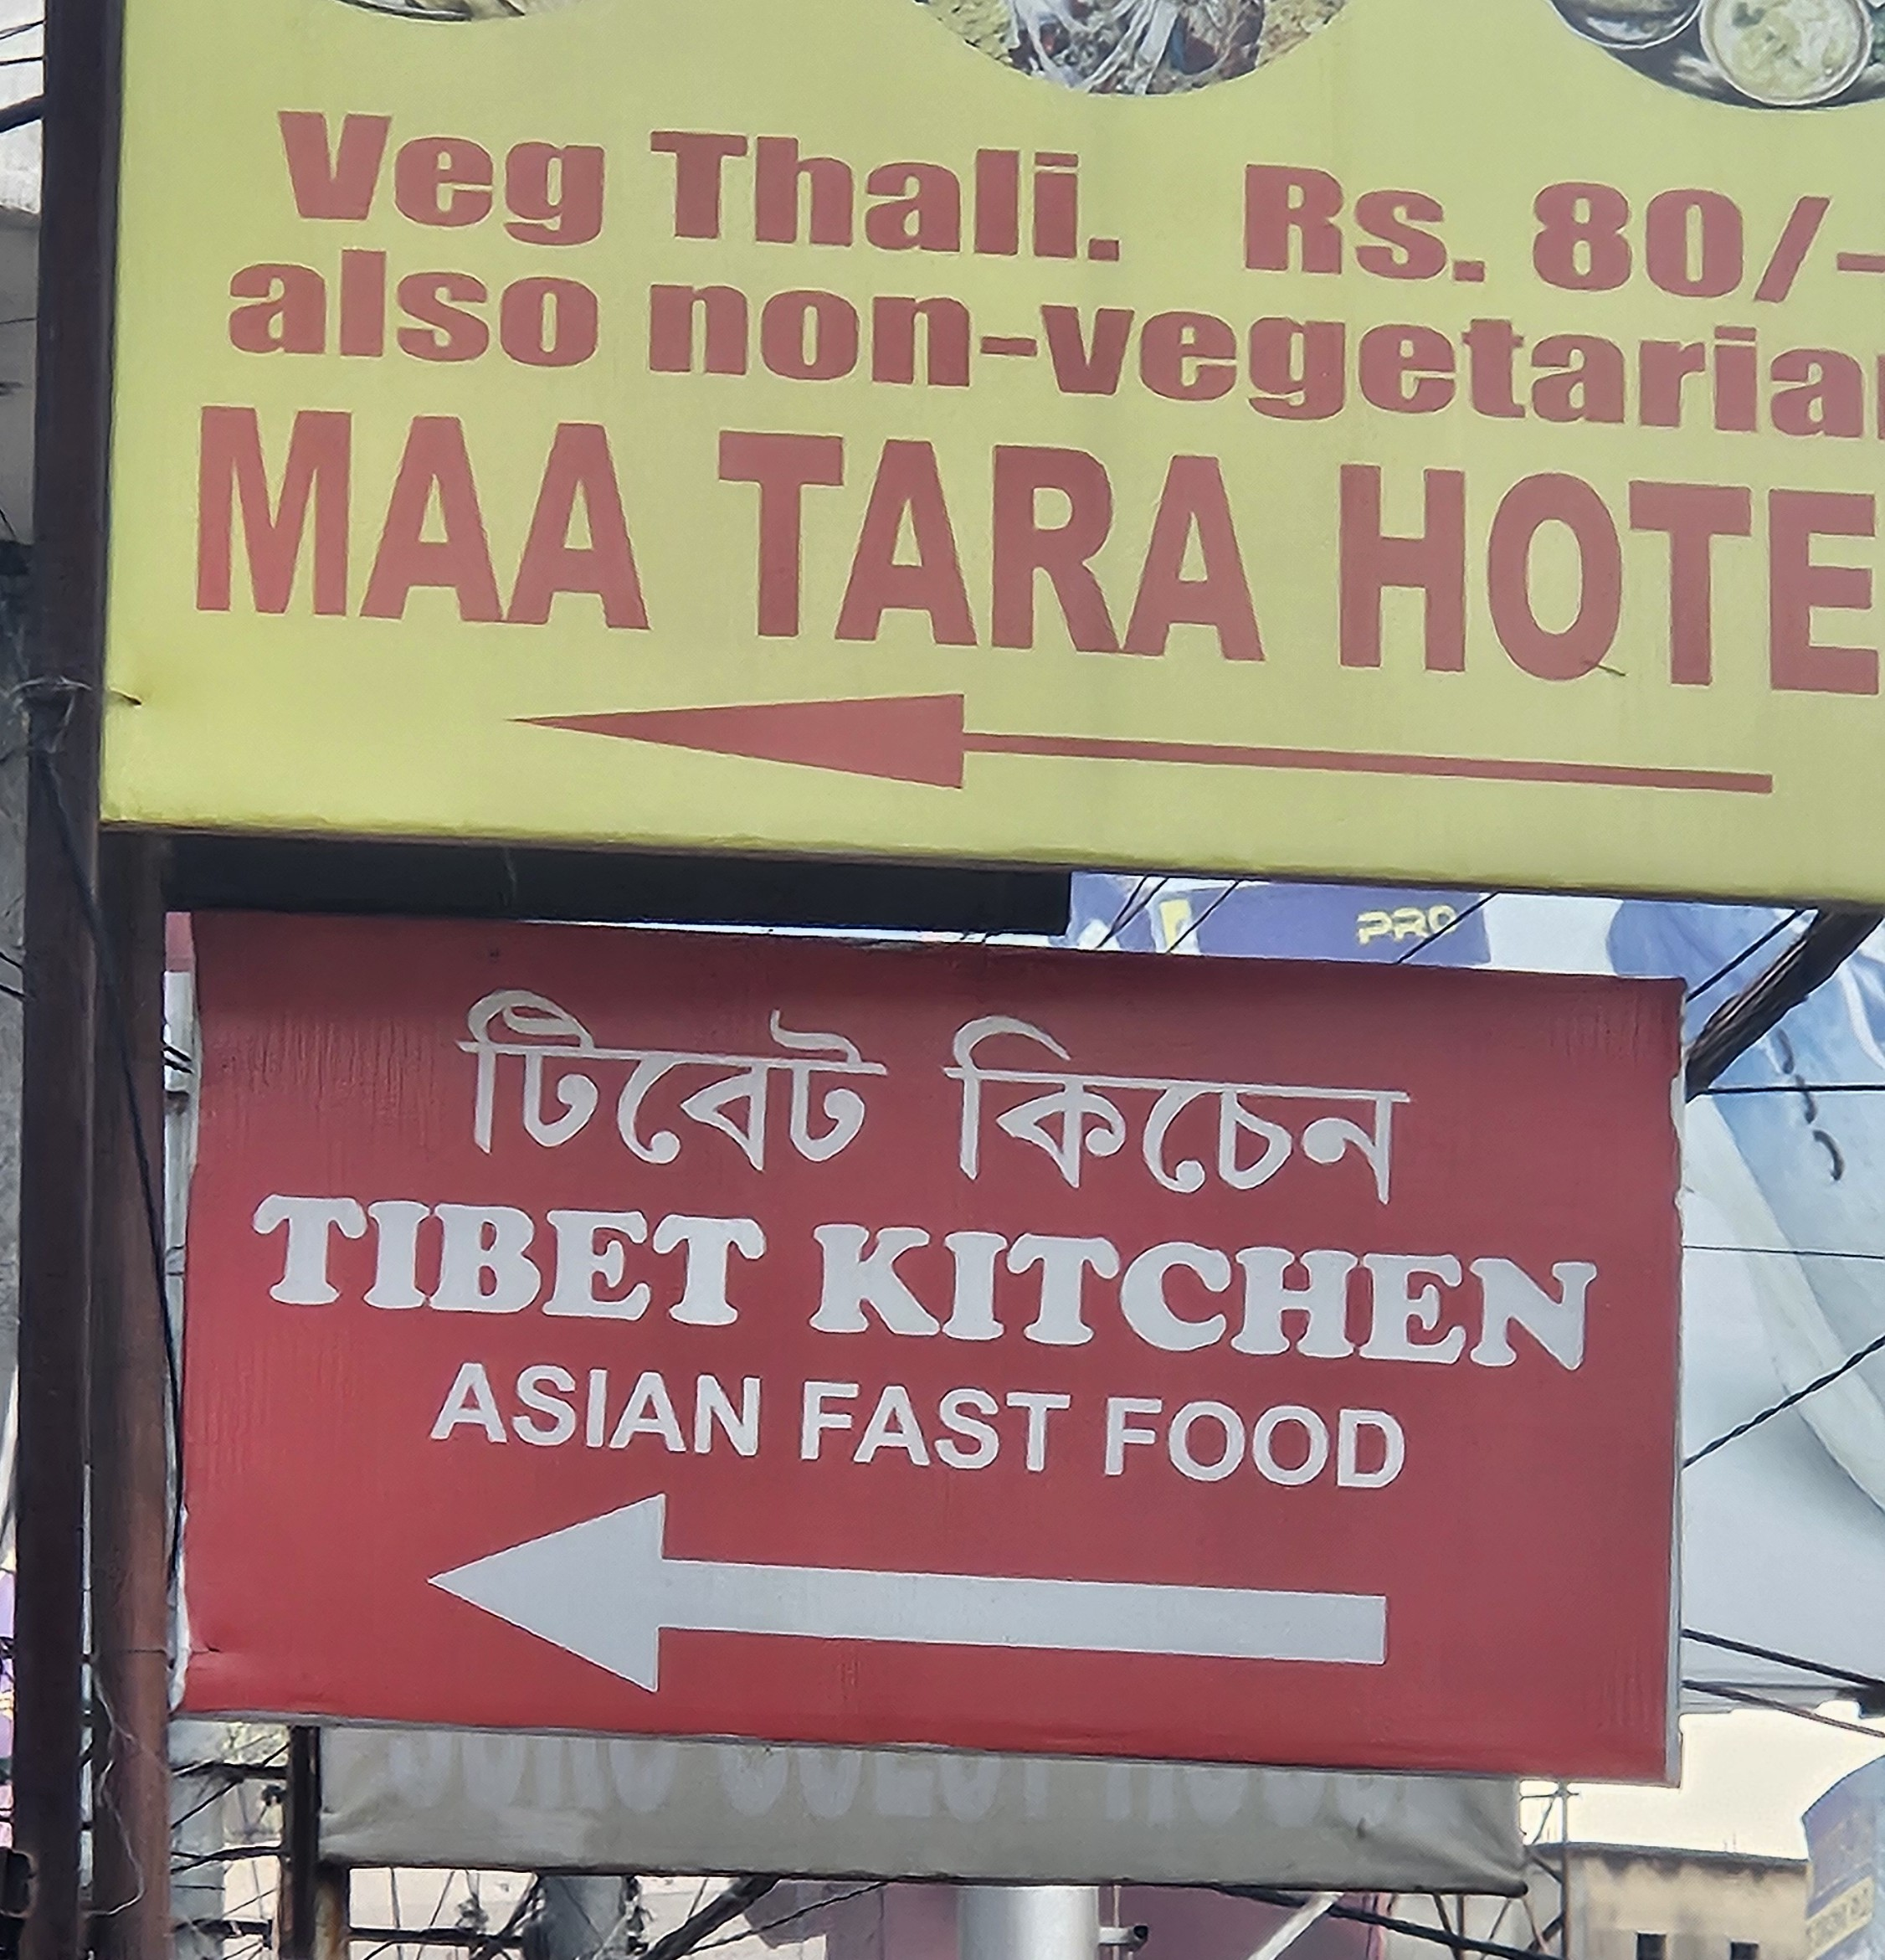
\includegraphics[width=\linewidth,height=1.45in,keepaspectratio]{figures/shop_signs_test1.jpg}\\
\small (b)
\end{minipage}
\caption{Real-scene examples: (a) Mohanbari road sign; (b) cropped view of the commercial signs. No prediction overlays are shown. Scoring used the original test images and only the three confirmed Assamese/shared-script words; Latin and tiny or partial background text were excluded.}
\label{fig:real-scenes}
\end{figure}

\subsection{Translation and Camera Measurements}
A translation-enabled replay of the two real images processed 198 frames in 60.53~s (3.271 frames/s). Mean detection and recognition times were 59.54 and 17.82~ms. Translation model loading took 6243.20~ms; four uncached generations averaged 138.57~ms (p95 187.34~ms), including one spurious OCR source. A hundred cache snapshots averaged 0.00464~ms. Outstanding translation work was drained after replay, and English rendering was excluded from this timing run. Generation latency and cache lookup cost are consequently reported separately from end-to-end English availability.

An instrumented CSI test attached source-buffer presentation timestamps (PTS), mapped through the GStreamer clock to host monotonic time. Three consecutive 20-second observations without translation published 763 frames in a scene with no detected text. Pooled source-PTS-to-shared-JPEG-publication age was 123.68~ms p50 and 143.44~ms p95; the startup-inclusive maximum was 932.85~ms. The timestamped transport includes host JPEG encoding, loopback transfer, latest-frame selection and the OCR/publication path. The measurement excludes calibrated exposure timing and HTTP/browser display.

For the translation-enabled live observation, the Mohanbari photograph was displayed to the CSI camera while the viewer remained running. All 60 one-second status snapshots contained text and an English output, with the existing translation cache retained. The processed-frame counter advanced by 496 over 59.28~s (8.367 frames/s). Peak sampled Python-worker RSS was 1651.92~MiB; mean CPU and GPU utilization were 50.60\% and 29.48\%, and mean module power was 9.18~W (Fig.~\ref{fig:live-resources}). This observation includes camera processing and English rendering. Table~\ref{tab:evidence} summarizes the embedded measurements.

\begin{table}[t]
\caption{Embedded execution and functional verification. The three-word accuracy check is scoped to two real photographs.}
\label{tab:evidence}
\centering\small
\begin{tabular}{p{0.53\columnwidth}p{0.36\columnwidth}}
\hline
Quantity & Result\\
\hline
Live camera with translation & 8.367 frames/s\\
Live peak sampled worker RSS & 1651.92 MiB\\
Live mean module power & 9.18 W\\
Translation generation mean / p95 & 138.57 / 187.34 ms\\
Detection / spotting H-mean & 1.00 / 1.00 (3 words)\\
Crop CER / exact word accuracy & 0\% / 3 of 3\\
Bilingual output consistency & 3 of 3\\
OCR model storage & 64.77 MiB\\
Jetson regression tests & 57 passed\\
\hline
\end{tabular}
\end{table}

\begin{figure}[t]
\centering
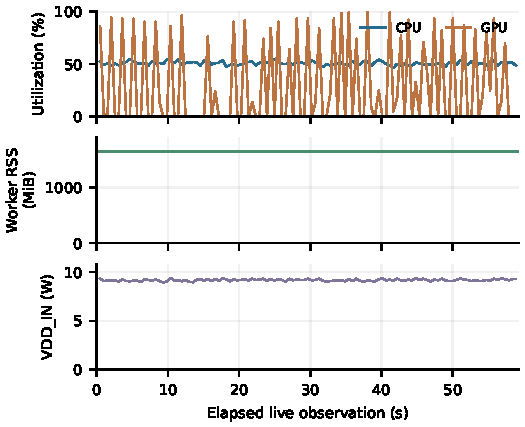
\includegraphics[width=\columnwidth]{figures/live_resources.pdf}
\caption{Live CSI resource observation with English translation enabled and the existing cache retained. CPU utilization is averaged across reported cores; RSS is the Python application worker; VDD\_IN is module power. This is a single warm-session observation, not a cold-start or sustained uncached-generation benchmark.}
\label{fig:live-resources}
\end{figure}

\subsection{Discussion}
The controlled replay quantifies the throughput advantage of CUDA for the same OCR workload. The live observation demonstrates integrated camera reading and English publication within a measured memory and power budget. Its higher throughput is not a speedup over replay: the scene density, JPEG input path and cache conditions differ. Cached translation is normal operation for persistent signage, but it does not characterize sustained uncached generation. The deployment thus separates recognition responsiveness from translation availability while retaining both outputs in one application.

The evaluation boundaries are specific: synthetic replay characterizes resource use; three real-image words provide functional checks; camera timing describes source PTS to publication; and live telemetry characterizes an existing-cache workload. Correlated frames and status snapshots are not independent accuracy samples. Generalization to unseen scenes, broader translation meaning preservation and oblique or curved text require a scene-disjoint annotated evaluation. The deployment uses direct resizing of approximately horizontal text crops, rather than the morphological/deskew preprocessing described in the conference manuscript.

\begin{samepage}
\section{Conclusion}
This letter extends our Assamese scene-text framework from model development to measured Jetson execution, combining ONNX detection and recognition with offline English translation and a continuous camera viewer. CUDA increases controlled OCR-replay throughput by 5.09 times over CPU execution. The translation-enabled live observation achieves 8.367 frames/s with 1651.92~MiB peak sampled worker RSS and 9.18~W mean module power under the recorded cache conditions. Together with real-scene functional checks and timestamped publication measurements, these results provide a reproducible characterization of the embedded reading system.

\end{samepage}
\balance
\begin{thebibliography}{13}
\bibitem{prior} M.~Enghi, A.~K.~Talukdar, and N.~Saikia, ``Design of a natural scene Assamese text recognition system,'' accepted manuscript, 11th National Conference on Computer Vision, Pattern Recognition, Image Processing and Graphics, LNMIIT, Jaipur, India, Jul.~22--24, 2026; proceedings not yet published.
\bibitem{synthtiger} M.~Yim, Y.~Kim, H.-C.~Cho, and S.~Park, ``SynthTIGER: Synthetic text image generator towards better text recognition models,'' in \emph{Proc. ICDAR}, 2021, pp.~109--124.
\bibitem{svtrv2} Y.~Du, Z.~Chen, H.~Xie, C.~Jia, and Y.-G.~Jiang, ``SVTRv2: CTC beats encoder-decoder models in scene text recognition,'' in \emph{Proc. IEEE/CVF ICCV}, Oct.~2025, pp.~20147--20156. [Online]. Available: \url{https://arxiv.org/abs/2411.15858}
\bibitem{parseq} D.~Bautista and R.~Atienza, ``Scene text recognition with permuted autoregressive sequence models,'' in \emph{Proc. ECCV}, 2022, pp.~178--196, doi: 10.1007/978-3-031-19815-1\_11.
\bibitem{rrc2015} D.~Karatzas \emph{et al.}, ``ICDAR 2015 competition on robust reading,'' in \emph{Proc. ICDAR}, 2015, pp.~1156--1160, doi: 10.1109/ICDAR.2015.7333942.
\bibitem{ctc} A.~Graves, S.~Fern\'andez, F.~Gomez, and J.~Schmidhuber, ``Connectionist temporal classification: Labelling unsegmented sequence data with recurrent neural networks,'' in \emph{Proc. ICML}, 2006, pp.~369--376, doi: 10.1145/1143844.1143891.
\bibitem{ort} ONNX Runtime, ``Execution providers,'' documentation. [Online]. Available: \url{https://onnxruntime.ai/docs/execution-providers/}. Accessed: Oct.~29, 2026.
\bibitem{jetson} NVIDIA, ``First picture with CSI or USB camera,'' Jetson tutorial. [Online]. Available: \url{https://developer.nvidia.com/embedded/learn/tutorials/first-picture-csi-usb-camera}. Accessed: Oct.~29, 2026.
\bibitem{quantization} B.~Jacob \emph{et al.}, ``Quantization and training of neural networks for efficient integer-arithmetic-only inference,'' in \emph{Proc. IEEE/CVF CVPR}, 2018, pp.~2704--2713, doi: 10.1109/CVPR.2018.00286.
\bibitem{indictrans2} J.~Gala \emph{et al.}, ``IndicTrans2: Towards high-quality and accessible machine translation models for all 22 scheduled Indian languages,'' \emph{Trans. Mach. Learn. Res.}, Dec.~2023. [Online]. Available: \url{https://openreview.net/forum?id=vfT4YuzAYA}
\bibitem{export} hari31416, ``IndicTrans2 Indic--English distilled 200M ONNX INT8,'' model repository. [Online]. Available: \url{https://huggingface.co/hari31416/indictrans2-indic-en-dist-200M-ONNX-int8}. Accessed: Oct.~29, 2026.
\bibitem{aoi} R.~D.~Yates, Y.~Sun, D.~R.~Brown~III, S.~K.~Kaul, E.~Modiano, and S.~Ulukus, ``Age of information: An introduction and survey,'' \emph{IEEE J. Sel. Areas Commun.}, vol.~39, no.~5, pp.~1183--1210, May~2021, doi: 10.1109/JSAC.2021.3065072.
\bibitem{tegrastats} NVIDIA, ``Tegrastats utility,'' \emph{Jetson Linux Developer Guide}. [Online]. Available: \url{https://docs.nvidia.com/jetson/archives/r36.4.3/DeveloperGuide/AT/JetsonLinuxDevelopmentTools/TegrastatsUtility.html}. Accessed: Nov.~25, 2026.
\end{thebibliography}
\end{document}
